%%%% IACR Transactions TEMPLATE %%%%
% This file shows how to use the iacrtrans class to write a paper.
% Written by Gaetan Leurent gaetan.leurent@inria.fr (2020)
% Public Domain (CC0)


%%%% 1. DOCUMENTCLASS %%%%
\documentclass[journal=tosc,submission, notanonymous]{iacrtrans}
%%%% NOTES:
% - Change "journal=tosc" to "journal=tches" if needed
% - Change "submission" to "final" for final version
% - Add "spthm" for LNCS-like theorems


%%%% 2. PACKAGES %%%%
\usepackage{lipsum} % Example package -- can be removed
\usepackage{blt}
\usepackage{tabularx}
\usepackage{graphicx}
\usepackage{xcolor}
\usepackage{url}


%%%% 3. AUTHOR, INSTITUTE %%%%
\author{Maximilian Heim\inst{1}}
\institute{
  University Albstadt-Sigmaringen, Albstadt, Germany, \email{MaximilianHeim@protonmail.com}
}
%%%% NOTES:
% - We need a city name for indexation purpose, even if it is redundant
%   (eg: University of Atlantis, Atlantis, Atlantis)
% - \inst{} can be omitted if there is a single institute,
%   or exactly one institute per author


%%%% 4. TITLE %%%%
\title{An Introduction to Return Oriented Programming}
%%%% NOTES:
% - If the title is too long, or includes special macro, please
%   provide a "running title" as optional argument: \title[Short]{Long}
% - You can provide an optional subtitle with \subtitle.

\begin{document}

\maketitle


%%%% 5. KEYWORDS %%%%
\keywords{ROP \and Return Oriented Programming \and ret2libc \and ret2lib \and ROP-Gadget \and Stack Overflow \and Buffer Overflow \and Binary Exploitation \and Cyber Security \and ASLR \and Address Space Layout Randomization \and NX \and DEP}


%%%% 6. ABSTRACT %%%%
\begin{abstract}
  Return Oriented Programming is a buffer overflow exploitation technique developed in 2007. Under certain circumstances it can provide arbitrary code execution on assembly level. Luckily the development of binary exploitation protections like stack canaries, bounds checking and ASLR made the effort required for developing an attack for that specific target and attacking the target too high to make it practicable in most cases, however, old soft-/hardware are still vulnerable and the mentioned protections have shown to be vulnerable themselves, with high enough reward ROP may be a devastating technique for black-hats.  
\end{abstract}


%%%% 7. PAPER CONTENT %%%%
\section{Introduction}
Return Oriented Programming, abbreviated ROP is a type of buffer overflow attack that has been published in 2007 by Hovav Shacham.~\cite{ropfirstpaper} and has become a widely known buffer overflow technique since. It has been developed to circumvent the NX-BIT protection that protects the stack from being executed. At the time of writing this paper modern techniques like stack carnaries and ASLR make these attacks hard and very time consuming on modern systems. That is not to say ASLR and stack canaries can not be broken by bruteforcing or side channels. Since there are millions of running systems with old hard-, firm- and software that is possibly vulnerable to these kinds of attacks it is still relevant to this day. The main idea in ROP is based on chaining return addresses to code just before a return and therefore allowing almost arbitrary cpu instructions to be chained.


\section{Gadgets}
\label{sec:gadgets}
\paragraph{Introduction}
On the x86 architecture the \Verb+ret+ instruction is defined to pop the return instruction pointer from the stack into the \Verb+eip+ register and redirect code execution to that memory address.~\cite{retx86} A ROP gadget consists of a few instructions (usually 1-3) that end on a \bltInlineVerb{ret}.

\paragraph{How to find Gadgets}
\label{par:ropgadget}
A gadget can be found by searching for \Verb+0xC3+ Bytes in the program. The instructions before then represent the code code that can be executed by injecting the addresses of these instructions. It is possible to search for gadgets with \Verb+objdump+ or \Verb+hexdump+, however, the tools specifically made for finding ROP gadgets are really easy to use and provide lots of customizability and features for finding the required gadgets. To name a few ROP gadget tools there is \Verb+ropper+, \Verb+ROPgadget+ and \Verb+pwntools+. For this paper the software \Verb+ROPgadget+ has been employed since i found it easy to use. \bltInlineVerb{ROPgadget} can be found in most package managers or can be downloaded directly from \url{https://github.com/JonathanSalwan/ROPgadget}. The gadgets can be extracted from the file with the following command~\cref{dumpallgadgets}. We can then use regular expressions or ROPgadget directly to search for the required gadgets.
\bltCommand{ropcommand.sh}{Exporting gadgets with ROPgadget}{dumpallgadgets}
This command produces an output with results similar to this.
\bltResult{dumppick}{Output of ROPgadget}{outputropgadget}
These are only 10 Lines out of the 8244 lines found by the tool though and i purposefully filtered out some good and bad ones for demonstration. It is clearly visible that many candidates for ROP can be found, even in a file with a relatively small size of 72 kB. Though most of these gadgets are not all that useful because they often modify a lot of registers, possibly messing up the desired state. In most cases we can find suitable candidates using regular expressions, this will be demonstrated later in this section~\cref{subsec:filtering}.
\paragraph{Overview of powerful gadgets}
\paragraph{pop}
\Verb+pop+ allows us to write arbitrary values into registers. For that we search for a \Verb+pop <reg>+ instruction inside our gadgets, in the payload we can then place the value that we want to insert after the address of the \Verb+pop+ instruction.~\cite{ropsla} If we can not find a suitable gadget we can try to get creative and achieve the desired state another way. For example if we want to modify \Verb+ecx+ but do not have a \Verb+pop ecx+ instruction available we could achieve it with something like this: \bltInlineVerb{xor ecx, ecx ; pop eax ; xor ecx, eax}. Provided that we have these gadgets available.
\paragraph{mov}
\Verb+mov+ allows us to read from memory, copy values from register to register and write arbitrary values into memory. In order to read from memory we have to search for a \bltInlineVerb{mov dword ptr <reg1>, [<reg2>]} instruction, we can then specify the memory address to read from in \bltInlineVerb{reg2}. In order to copy a value from register to register we have to search for a \bltInlineVerb{mov <reg1>, <reg2>} gadget. In order to write to memory we have to search for a \bltInlineVerb{mov dword ptr [<reg1>], <reg2>} instruction inside our gadgets, we can then specify the value in \bltInlineVerb{reg2} and the address in \bltInlineVerb{reg1}, given there is a way to modify both registers.
\paragraph{arithmetics, boolean algebra}
Arithmetic operations like \Verb+add+, \Verb+sub+, \Verb+inc+ and \Verb+xor+ can be useful to bring registers into our desired state.~\cite{ropsla} For that we search for the corresponding gadget with the required operands. For example \Verb+xor+ can be used to clear a register or copy its contents. It often occurs in the following forms: \bltInlineVerb{xor eax, eax} or \bltInlineVerb{xor eax, edx}. The first case clears the register since \Verb+xor+ computes a non-equivalence, formally $a \oplus a = 0$ and the second one copies the value of the 2nd operand into the 1st operand when the target register is \Verb+0x00+ since \Verb+0x00+ is the neutral element of the \Verb+xor+ operation, formally $a \oplus 0 = a$.
\paragraph{int 0x80}
\Verb+int+ stands for interrupt, the interrupt \bltInlineVerb{int 0x80} causes a system call to be executed. System calls are kernelspace programs/operations that require higher privileges than what is available in a userspace program. Examples for system calls include io and \Verb+execve+ which allows to execute arbitary programs. In combination with \Verb+pop+, \Verb+mov+ and other instructions we can specify the concrete system call.~\cite{ropsla} One of the most powerful system calls for blackhats is bash since it allows permanently implementing malware or gain insight into files, it can be called with the argument \Verb+/bin/sh+. This will be demonstrated in~\cref{sec:attack}.
\subsection{Filtering the gadgets}
\label{subsec:filtering}
\paragraph{Introduction}
In order to find the required gadgets we can use the tools directly or we can use regular expressions. In order to make this paper more general and easy to replicate i will be using regular expressions to find the desired gadgets.
\paragraph{Gadgets and their corresponding Regular Expression}
The following table describes what regex we can use to find the gadgets required for the attack.
\begin{itemize}
\item pop edx  $\rightarrow$ \bltRegex{\^{}.\{0,20\}pop edx.\{0,20\}ret\textbackslash{}n}
\item int 0x80  $\rightarrow$ \bltRegex{\^{}.\{0,20\}int 0x80\textbackslash{}n} 
\item xor eax, eax  $\rightarrow$ \bltRegex{\^{}.\{0,20\}xor eax, eax.\{0,20\}ret\textbackslash{}n} 
\end{itemize}
for all of these regular expressions there were gadgets for the given program in~\cref{sec:attack}. If there are no results the amount of possible characters before or after the gadget can be increased until results show up. It is however desirable to have gadgets with as few and noninterfering instructions as possible, if this is accomplished we can almost use the instructions we found like in assembly. Gadgets which do multiple things at once however can mess up the desired state and break the payload so it is important to thoroughly analyze the gadgets before generating the payload.

\section{Theory}
\subsection{Stack}
The following graphic~\cref{fig:stack} is an illustration of how the stack changes when injecting the payload. The buffer first has to be filled. In binary exploitation the letter \Verb+A+ is used for that most of the time, it has an easy to identify hexadecimal value of \bltInlineVerb{0x41}. It is important to note that without any special compiler options the stack will be aligned in \bltInlineVerb{dword}'s/16 Byte blocks. because of that the buffer has to be filled with more bytes than the buffer holds if $s \mod 16 \neq 0$ holds true, s being the buffer size in Bytes.
\newpage
\begin{figure}[h!]
  \centering
  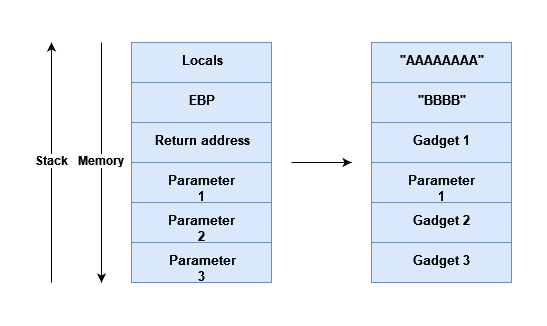
\includegraphics[width=0.79\textwidth]{stackropoffsec.png}
  \caption{The stack when injecting the payload}
  \label{fig:stack}
\end{figure}
\subsection{ROP Runtime Behaviour}
The following graphic~\cref{fig:executionatruntime} illustrates how the gadgets get executed once the instruction pointer \bltInlineVerb{eip} points to the \bltInlineVerb{ret} in \bltInlineVerb{main}. Once this happens the execution gets redirected to the first gadget and executes the instructions in it. As soon as \bltInlineVerb{eip} points to the \bltInlineVerb{ret} in the 1st gadget the address of the 2nd gadget is \bltInlineVerb{pop}'d into \bltInlineVerb{eip} and execution continues there, from there the same thing happens again until execution reaches the end of the last gadget.
\begin{figure}[h!]
  \centering
  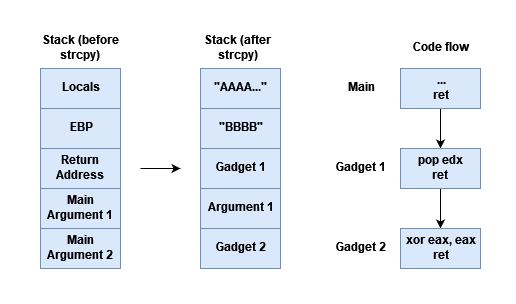
\includegraphics[width=0.95\textwidth]{Ropchaineffect.png}
  \caption{The stack when injecting the payload}
  \label{fig:executionatruntime}
\end{figure}
\section{Attack}
\label{sec:attack}
\subsection{Target Program}
\paragraph{Target Program}
The following program is the target of our attack, it uses a command line argument to provide the payload and \Verb+strcpy+ for the buffer overflow, overwriting the return address after the 8 Byte buffer.
\bltCode{vuln.c}{c}{The Target Program}{thetargetprogram}
\paragraph{Compilation}
We compile the target program with the following command. There are several important options given in this command. Most importantly the \bltInlineVerb{-fno-stack-protector} option disables stack canaries which would otherwise directly terminate the program when the canary is overwritten. The \Verb+-m32+ option compiles the binary as a 32 Bit executable, this makes the attack easier. The \Verb+-static+ option makes the binary statically linked. Without this option there are only 50 gadgets available, considering most of them are not useful for our attack it is practically impossible to perform the attack with just these gadgets. The \Verb+-static+ option includes the \Verb+libc+ library in the executable, increasing the gadget count to over 8000. However, it is possible to determine the address of the dynamically linked library at runtime and adding an offset for each gadget to this address. This has been described by Saif El-Sherei~\cite{el-sherei} but will not be further discussed in this paper.
\bltCommand{compilation.sh}{The compliation command}{thecompilationcommand}
\subsection{Phases of developing the attack}
\paragraph{Phases}
The attack consists of several phases
\begin{enumerate}
  \item Specify attack, analyze necessary setup to be done.~\cref{par:goal}
  \item Extract gadgets using tools, e.g. ROPgadget~\cref{par:ropgadget}
  \item Determine how many words are needed to override the base pointer \Verb+ebp+~\cref{par:padding}
  \item Determine position of a writable data segment~\cref{par:data}
  \item Generate payload with the extracted gadgets based on the specification in step 1.~\cref{par:genthepayload}
  \item Insert payload into target using a vulnerability~\cref{par:injthepayload}
\end{enumerate}
\subsection{The attack}
\paragraph{Specification and abstract payload}
\label{par:goal}
After specifying the goal and possibly simplifying it we have to determine the required program state. For the example in this paper we want to open a shell, for that the simplest way is to execute an \bltInlineVerb{execve} system call. The following program state~\cref{fig:stateforint} has to be achieved so the interrupt \bltInlineVerb{int 0x80} causes a shell to be opened.~\cite{pixis}~\cite{proggen-rop}
\begin{figure}[h]
  \centering
  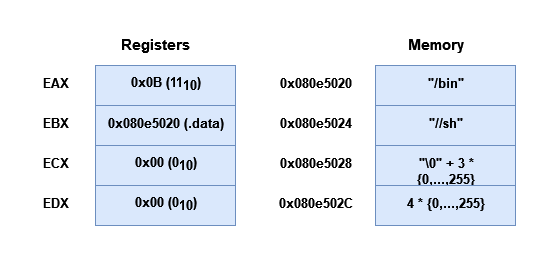
\includegraphics[width=0.95\textwidth]{requirementstackmemory.png}
  \caption{Required Program State for the execve Syscall}
  \label{fig:stateforint}
\end{figure}
\paragraph{Extract gadgets}
The gadgets can be extracted like described in~\cref{sec:gadgets}
\paragraph{Determine the padding}
\label{par:padding}
Compilers optimize stack alignment and without providing options to change that the simplest way to determine the padding required is to test the program until it crashes with a payload increasing by 1 word in each iteration. This can be automated in a Python script~\cref{code:determinewordcount}. This script applies the method mentioned above with the \bltInlineVerb{os.system} function. The return value of that function is the exit code of the program that has been executed and is either \Verb+0+ when the execution ended without any errors and non \Verb+0+ when an error or exception occured during startup or runtime. This means we can increase the input by \bltInlineVerb{"AAAA"} in each iteration until the return value is non zero. At this point the base pointer \bltInlineVerb{ebp} has been overridden causing the program to crash. Now reducing the padding by 1 word results in the correct amount.
\bltCode{determinewordcount.py}{python}{A Python Script to Determine the Required Words}{code:determinewordcount}
\paragraph{Determine the address of a writable segment}
\label{par:data}
The segments in a binary can be read only or writable. It is possible to determine wether a segment is read only with \bltInlineVerb{objdump -h}. However, the following~\cref{command:finddatasegment} bash command can be used to find the address of the data segment. The data segment contains static and global variables. Since the target program does not have any global or static variables we can override this segment with arbitrary character sequences. In 
\bltCommand{objdump.sh}{Determine the Address of .data}{command:finddatasegment}
\paragraph{Generating the payload}
\label{par:genthepayload}
There are many ways to generate the payload, the most common and simple method is with pythons \bltInlineVerb{struct.pack} function.~\cite{proggen-rop} The following example~\cref{code:howtopack} illustrates how to generate a payload with \bltInlineVerb{pack}.
\bltCode{pack.py}{python}{How to use struct.pack}{code:howtopack}
Now that all requirements are met the payload can be constructed.
\subparagraph{/bin//sh}
The first step is to write \bltInlineVerb{/bin//sh} into the \bltInlineVerb{.data} segment. This implies the use of the \bltInlineVerb{mov} function. Ideally the registers used should either be \bltInlineVerb{eax}, \bltInlineVerb{ebx}, \bltInlineVerb{ecx} or \bltInlineVerb{edx} since these registers provide the easiest access, usually with multiple \bltInlineVerb{pop} gadgets in an executable. After checking the gadgets the following seemed like the best gadget: \bltInlineVerb{0x08080742 : mov dword ptr [edx], eax ; ret}. Locating the \bltInlineVerb{pop} instructions for these 4 registers was simple and yielded: \bltInlineVerb{0x080ac76a # pop eax ; ret}, \bltInlineVerb{0x08049022 # pop ebx ; ret}, \bltInlineVerb{0x08054f5b # pop ecx ; add al, 0xf6 ; ret} and \bltInlineVerb{0x0808b285 # pop edx ; xor eax, eax ; pop edi ; ret}. The 3rd gadget adds a number to the \bltInlineVerb{eax} register and the 4th gadget \bltInlineVerb{xor}'s it. For the sake of this attack this is not a problem since we can simply modify \bltInlineVerb{eax} last. The 4th gadget also \bltInlineVerb{pop}'s a value into \bltInlineVerb{edi} which does not interfere with this attack, it just means that we have to provide an arbitary word after the parameter for \bltInlineVerb{pop edx}. With these instructions it is possible to write \bltInlineVerb{"/bin//sh"} into the \bltInlineVerb{.data} segment. Once a string is written into memory it still needs to have a \bltInlineVerb{0x00} Byte added after it, that is because some \bltInlineVerb{string.h} functions use the \bltInlineVerb{0x00} Byte to identify the end of a string. This means that depending on the implementation of the target it is important to not insert any \bltInlineVerb{0x00} Bytes into the payload otherwise the buffer does overflow fully. In most cases we can still write \bltInlineVerb{0x00} Bytes into registers or into memory. This can be accomplished by \bltInlineVerb{xor}'ing a register with itself and then copying that value into a register or into memory. In order to write a \bltInlineVerb{0x00} Byte after the string we can \bltInlineVerb{xor} the \bltInlineVerb{eax} register with \bltInlineVerb{0x08050a08 # xor eax, eax ; ret}. After that we simply have to copy it again.
\subparagraph{Initializing the registers}
As seen in~\cref{fig:stateforint} we first need to write the address of \bltInlineVerb{/bin//sh} into \bltInlineVerb{ebx}, this can simply be done with the \bltInlineVerb{pop ebx ; ret} gadget. Then we need to clear \bltInlineVerb{ecx} and \bltInlineVerb{edx}. For clearing \bltInlineVerb{edx} the gadget \bltInlineVerb{0x0807b179 # xor edx, edx ; mov eax, edx ; ret} is a good candidate, since it only modifies \bltInlineVerb{eax} apart from the desired effect. There were no \bltInlineVerb{xor ecx, ecx} or \bltInlineVerb{mov ecx, <reg>} gadgets that ended on a return so \bltInlineVerb{ecx} was just set to point at the null pointer after the \bltInlineVerb{/bin//sh} string, making the provided argument list empty. The last step to set up the \bltInlineVerb{execve} system call is to set \bltInlineVerb{eax} to \bltInlineVerb{11}/\bltInlineVerb{0x0B}. For that we can use the \bltInlineVerb{0x08050a08 # xor eax, eax ; ret} gadget from before to set \bltInlineVerb{eax} to \bltInlineVerb{0x00} and then increment it 11 times with \bltInlineVerb{0x0809d0ae # inc eax ; ret}.
\subparagraph{Interrupt}
In the end the \bltInlineVerb{0x080499b2 # int 0x80} interrupt gets called. If the state got initialized correctly \bltInlineVerb{/bin//sh} gets executed.
\subparagraph{Constructing the payload}
From all the previous steps the payload got constructed with python~\cref{code:payloadbinsh}. As seen in the example we can define all the addresses, gadgets and other parameters as variables and reuse them in the \bltInlineVerb{pack} calls, this way changing a gadget only requires one value to be changed. The different
\bltCode{payload.py}{python}{Payload to open /bin/sh}{code:payloadbinsh}
\paragraph{Injecting the payload}
\label{par:injthepayload}
How the payload gets injected depends on the target. For the example in this paper the payload can be injected using the following commands~\cref{command:injthepayload}.
\bltCommand{inject.sh}{Injecting the payload}{command:injthepayload}
\section{Results}
\paragraph{Attack}
After injecting the generated payload from \cref{sec:attack} as a command line argument the program opened a shell from which we can use privilege escalation techniques in order to completely compromise the system.
\begin{figure}[h]
  \centering
  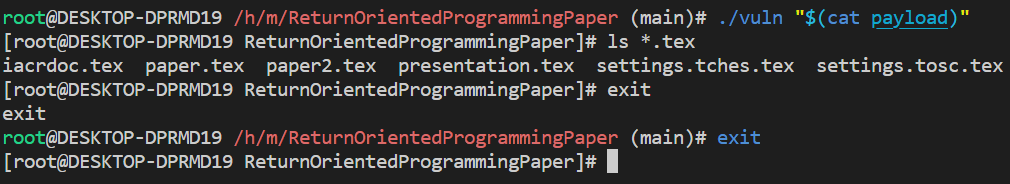
\includegraphics[width=0.95\textwidth]{ROPdone.png}
  \caption{Shell Opened iwith ROP}
  \label{fig:success}
\end{figure}
The only protections that had to be disabled were stack canaries and ASLR. It is likely that there are systems still in use today which are vulnerable to this kind of attack due to not having these protections or the protections themselves being attackable. Since it allows almost arbitrary code execution it is very important to identify these devices and patch or replace them.
\paragraph{ASLR}
The information wether ROP works with ASLR enabled is inconsistent. While trying this attack with \bltInlineVerb{/proc/sys/kernel/randomize_va_space} set to \bltInlineVerb{2} meaning full randomization the attack still seemed to work. The inconsistent information probably arises due to different approaches being used. With executables that have PIE enabled ROP is still possible but only with ASLR disabled~\cite{el-sherei}. With the compiler options used for this example PIE is disabled and ASLR seems to have no effect on the exploit. This is because the ASLR settings \Verb+1+ and \Verb+2+ only randomize shared libraries and PIE binaries~\cite{rny}, since the program has been compiled with the \bltInlineVerb{-static} option, which implicitly compiles the program to not be position independent, ASLR is not being used, even when activated.

\section{Protection}
\paragraph{Stack canaries}
Stack canaries are one of the most effective approaches against ROP, they are enabled by default and prevent most forms of buffer overflows, however, stack canaries can be based on a small entropy pool and can therfore be bruteforced with an effort significantly smaller than regular bruteforcing. Depending on the target it can still be profitable and possible to bruteforce it even with a big entropy pool and high randomness.
\paragraph{NX}
The activation of the NX bit has no effect on ROP since the program never executes code outside the segments marked with the \bltInlineVerb{CODE} flag like in a classical stack overflow attack.~\cite{ropsla}
\paragraph{ASLR}
According to a paper by Hovav Shacham et al. ASLR is a good protection against ROP in 64 bit binaries assuming no side channel leakage since 40 bit are available for randomizations of the libraries and code locations, however, 32 Bit binaries only use 16 Bit for randomization. Because of that they were able to perform a buffer overflow attack like ret2libc on an Apache server with an average of 216 seconds.~\cite{aslr}
%%%% 8. BILBIOGRAPHY %%%%
\bibliographystyle{alpha}
\bibliography{refs}
%%%% NOTES
% - Download abbrev3.bib and crypto.bib from https://cryptobib.di.ens.fr/
% - Use bilbio.bib for additional references not in the cryptobib database.
%   If possible, take them from DBLP.
\end{document}
